\newpage
\section{Results and Analysis}

% SECTIONS
% Results

% Analysis
% What the hell is going on? Why are the strongest results in violation of the order? (Is the order interpreted in the wrong direction?...)

% Ablation study, Sensibility analysis of hyperparameters
% Weaknesses (in relation to assumptions)

% Selecting only compliant relations: there's just very few left, they happen to be wrong?


% ROCs
We evaluate the methods using receiver operating characteristic (ROC) curves. The methods assign a score to every causal relation. The ROC curves plot how the number of true positives and false positives change for different thresholds on this score. Each method only assigns a score to some relations. If we require predictions beyond this point, we can only guess randomly. 

The ROC curves in Figure \ref{fig:7:rocshort} are discussed in detail in this section. For each method, we aggregated continuous predictions and evaluated on the absolute score ground-truth. The curves for other settings are shown in Appendix \textbf{APPENDIX}. The conclusions that we draw here are applicable to the other settings as well. 

ROC curves show the number of true positives on the x-axis versus false positives on the y-axis. Good methods rise quickly. Figure \ref{fig:7:rocshort} shows different ways to evaluate the same methods. Each column represents a different ground-truth threshold. This threshold indicates the percentage of top scoring relations that are considered to be true. Each row represents an evaluation filter. Methods are evaluated on the full dataset, the intervention table, and the relations that are explicitly compliant to the inferred order and test variable position. After the last prediction of a method, we indicate random guessing with a dashed line.

We first recapitulate the main findings of \citet{versteeg2019boosting} about the baseline methods. Then we compare order-based LCD to them. Finally we discuss the effect of preselection to our method.

\begin{figure}[h]
    \centering
    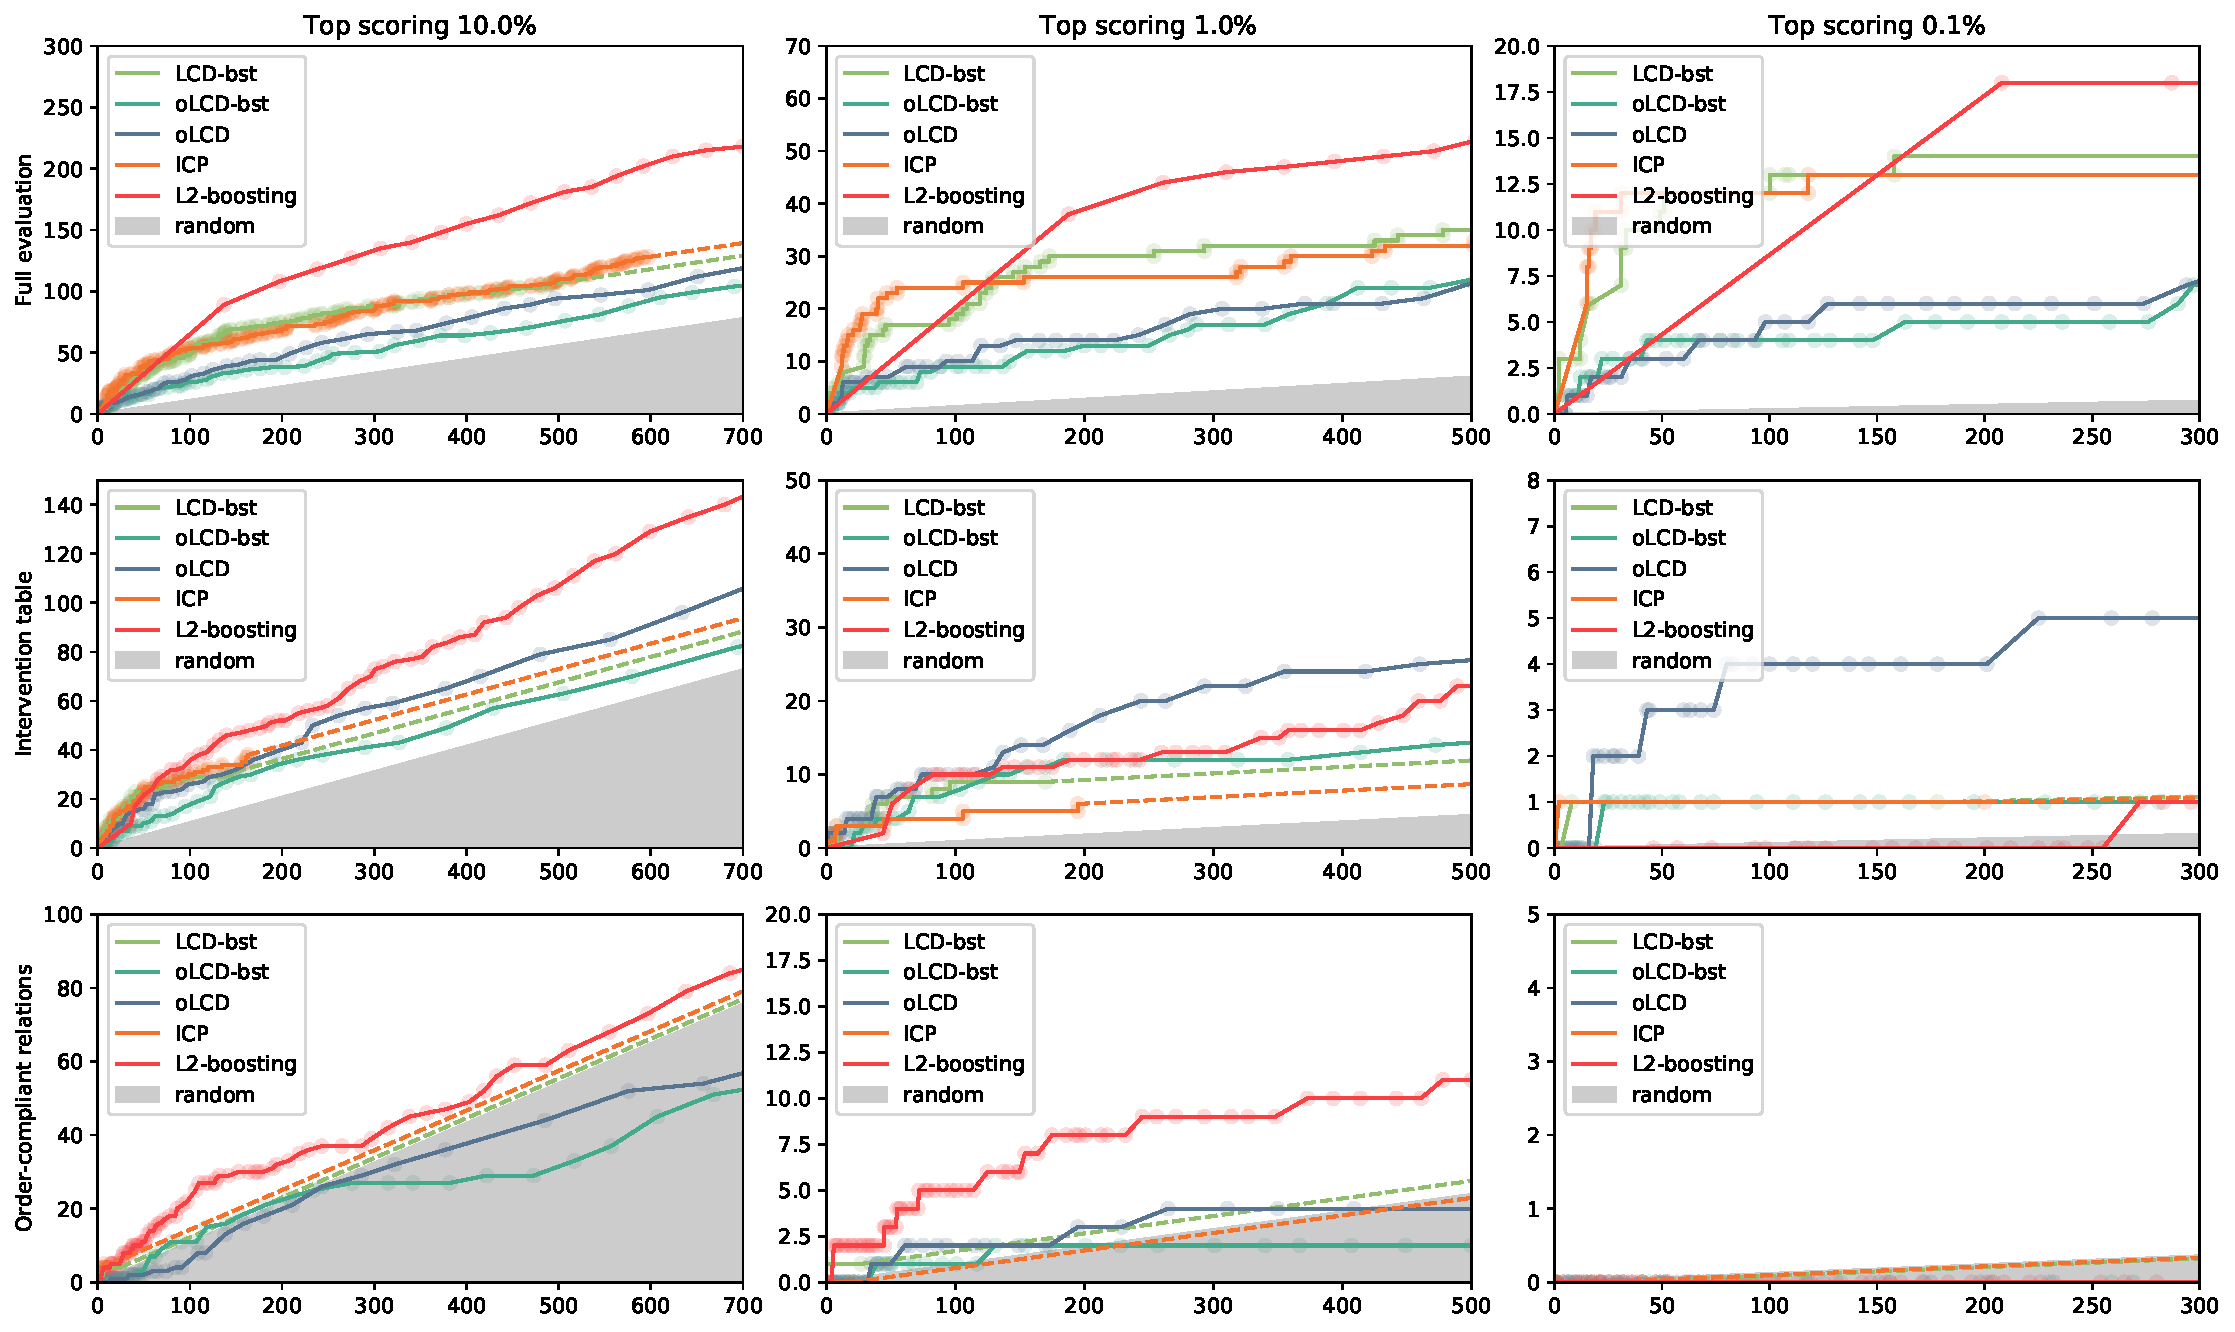
\includegraphics[width=\textwidth]{ROC_filter_threshold_absgt_scorespred_short.pdf}
    \caption{Partial ROC curve using the absolute ground-truth with aggregation of continuous scores.}
    \label{fig:7:rocshort}
\end{figure}

\subsubsection{Baselines}

% ICP/LCD is more fine-grained at start
Since we compare order-based LCD to the baseline methods of \citet{versteeg2019boosting}, we first summarize their findings\footnote{The exact ROC curves of that paper can be found in Appendix \textbf{APPENDIX}, in the top row of Figure \textbf{FIGURE}}. 226 relations are predicted in all subsamples by the non-causal L$_2$-boosting baseline. They are shown as the first point in the ROC curves. When we wish to use this method to make fewer predictions, we can only guess randomly within this set. The predictions of ICP and LCD are more fine-grained, because their 200 strongest predictions contain multiple confidence levels. LCD and ICP have many more true positives in their top 70 than L$_2$-boosting, as can be seen in the top row of Figure \ref{fig:7:rocshort}. This is where the non-causal baseline is beaten.

% LCD is largely explained by L2
Moreover, \citet{versteeg2019boosting} investigate the impact of L$_2$-boosting preselection on LCD. Preselection improves the method significantly. Preselection is what makes LCD comparable to ICP, being computationally less expensive. LCD can be interpreted as a causal filter on the non-causal L$_2$-boosting baseline. The baseline works surprisingly well on its own. The LCD conditions are a causal check that filter out mistakes of in the baseline, specifically causation in the opposite direction and confounding.

% LCD does not make many predictions
As a last remark, we note that LCD with preselection does not make many predictions. Only 608 relations of 126.103 preselected relations are assigned a non-zero score. When we are interested in beating the L$_2$-boosting baseline, this does not matter. The baseline is only beaten in the first 70 predictions. However, if we want to select a large number of relations, this is a restriction.


\subsubsection{Order-based LCD}

% Direct comparison: worse
Order-based LCD performs significantly worse than the baselines when evaluated on the full data set. The strongest predictions contain more false positives than LCD and ICP. 

Better results can be seen when we evaluate on the intervention table. Order-based LCD beats the non-causal baseline in the strongest predictions, and stays comparable after that. LCD and ICP perform slightly worse. 

When we only evaluate on relations that explicitly comply to the inferred order, order-based LCD does not perform better than LCD or ICP. This is unexpected, since the order-based context should be most informative for these relations. Instead, comparing to the results on the intervention table, it seems like the performance is better on relations that violate the order.

What is most important to the causal inference, is that the data points in which a true ancestor is intervened on, are associated with context value 1. Many of the remaining context values should be 0, such that the two clusters can be distinguished and the causal relation can be identified. Since the number of true ancestors may not be large, we are allowed to make many mistakes in the context.

% positions are skewed to the back
Position inference is constructed such that the positions generally tend to be estimated later in the order than they actually are. Therefore, what may seem like an order violation may just be a conservative estimate of the position.

% 'wrong order' does not create wrong prediction; order and position is messy
More importantly, the order inference and position inference algorithms are far from perfect. Many relations that are taken as order violation may be compliant to the real order in the underlying graph. Although a messier order and position reduces recall, it is not necessarily harmful to the precision. The context may not be very informative of the order, it still satisfies the exogeneity assumption. The LCD conditions imply an ancestral relation regardless of the interpretation of the context values. Still, a more informative context is desirable, since we expect LCD to be able to detect more of the true relations.


% Boosting bad
\subsubsection{Preselection}
Contrary to the results of the original LCD algorithm, L$_2$-boosting preselection does not have a clear benefit to order-based LCD. In fact, in the evaluation on the intervention table it reduces performance. 

We can interpret the boosting baseline as a filter on LCD. In the case of the intervention table evaluation, this filter takes out true strong predictions, indicating that order-based LCD uses information that is not found at all by the non-causal baseline. This interpretation is the reverse from that of \citet{versteeg2019boosting}, who interpret LCD as a filter on L$_2$-boosting that uses causal information to select the strongest relations beating boosting in the first predictions. 


% More predictions, some information about top 1000+? Some causal info not in L2?




% If accidentily right, still predicts right (accidentilly wrong, doesn't predict)
% What is actually relevant according to the hypothesis: interventions on ancestors should be in cluster C=1, many of the remainder should be in C=0. This can still be the case when order and position are messy, especially when the graph is sparse and there aren't many ancestors.

% Int filter: unfair comparison

% Comparable to L2 further on, without requiring it as preselection. (much further, on int data, even better without boosting)




% - Versteeg improves within the strongest prediction of L2: 226 relations are predicted in all subsamples; large part explained by L2 -> here it doesnt really matter
% - We present results of one setting (abs, cont) here, results of this setting of normal LCD are comparable to their setting (std, disc). We shortly discuss differences in the end.
% - LCD is a filter on L2-boosting
% - normal LCD does not predict much, but its strongest predictions are better than just taking L2
% - orderLCD makes more predictions (see wider ROCs in appendix). The weaker predictions are better than LCD which has to resort to random guessing. Worse than L2, so not that useful in itself but interesting direction of research.
% - orderLCD only improves over L2 in two settings
% - boosting doesn't help, and is harmful on intervention table evaluation!

% The intervention table contains the relations in explicit violation of the order (inferred position is later than target in order), relations explicitly complying to the order (inferred position is earlier than target in order), and relations for which the compliance is unknown (target is also in test split). Compared to the results on the intervention table, it may seem like order-based LCD performs better on explicit order violations than on compliant relations. 

% Versteeg: top 20 is pretty good, deBoer: top 400 is bad but comparable to baseline


